% !TEX root = ../beamer.tex

\begin{frame}
    \frametitle{Our Procedure}
    \begin{itemize}
   \item Agile software development using the Scrum methodology
   \item Scrum board with user stories and responsibilities
    \end{itemize}
    \vfill
    \begin{center}
		\begin{tikzpicture}
			\node[fill=white, draw, drop shadow] {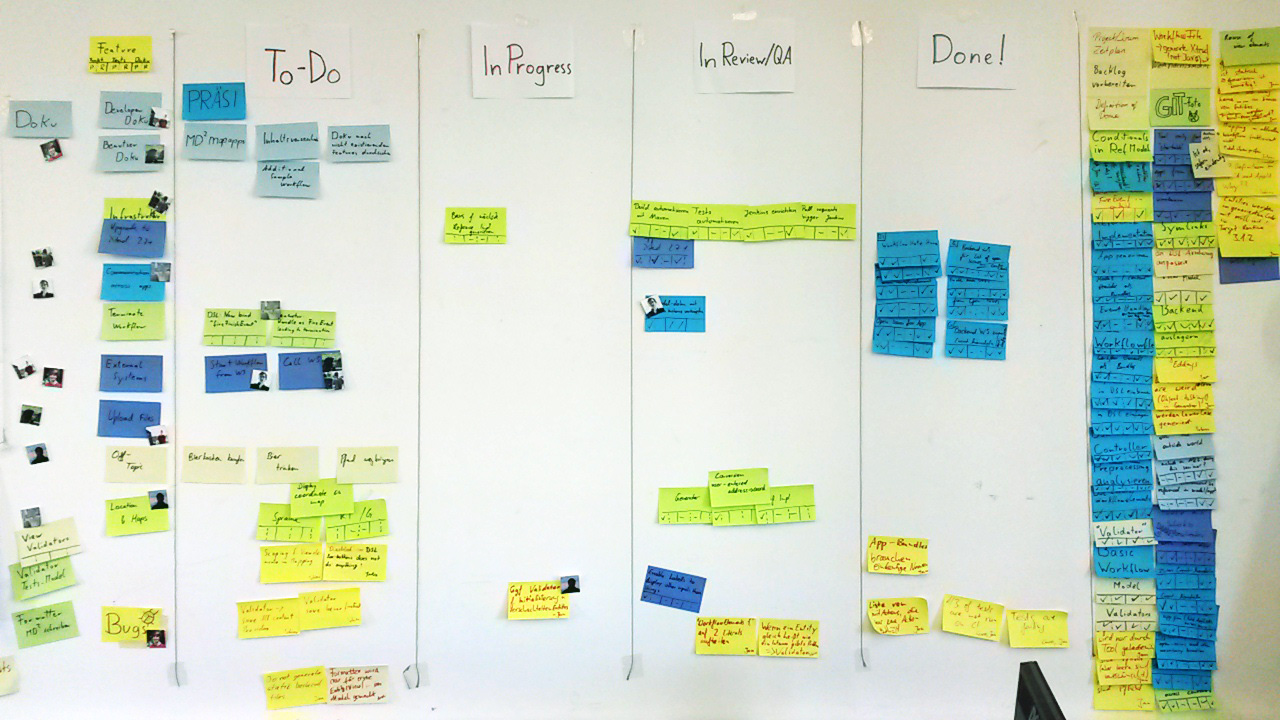
\includegraphics[height=40mm]{images/scrumboard}};
		\end{tikzpicture}
    \end{center}
\end{frame}

%-----------------------------------------------------------------------------------

\begin{frame}
	\frametitle{Our Scrum Board}
    \begin{figure}
	    \begin{center}
	        \pgfimage[height=60mm]{images/scrum.png}
	    \end{center}
	\end{figure}
\end{frame}

%-----------------------------------------------------------------------------------

\begin{frame}[plain]
	\frametitle{Bugs}
    \begin{center}
		\begin{tikzpicture}
			\node[fill=white, draw, drop shadow] {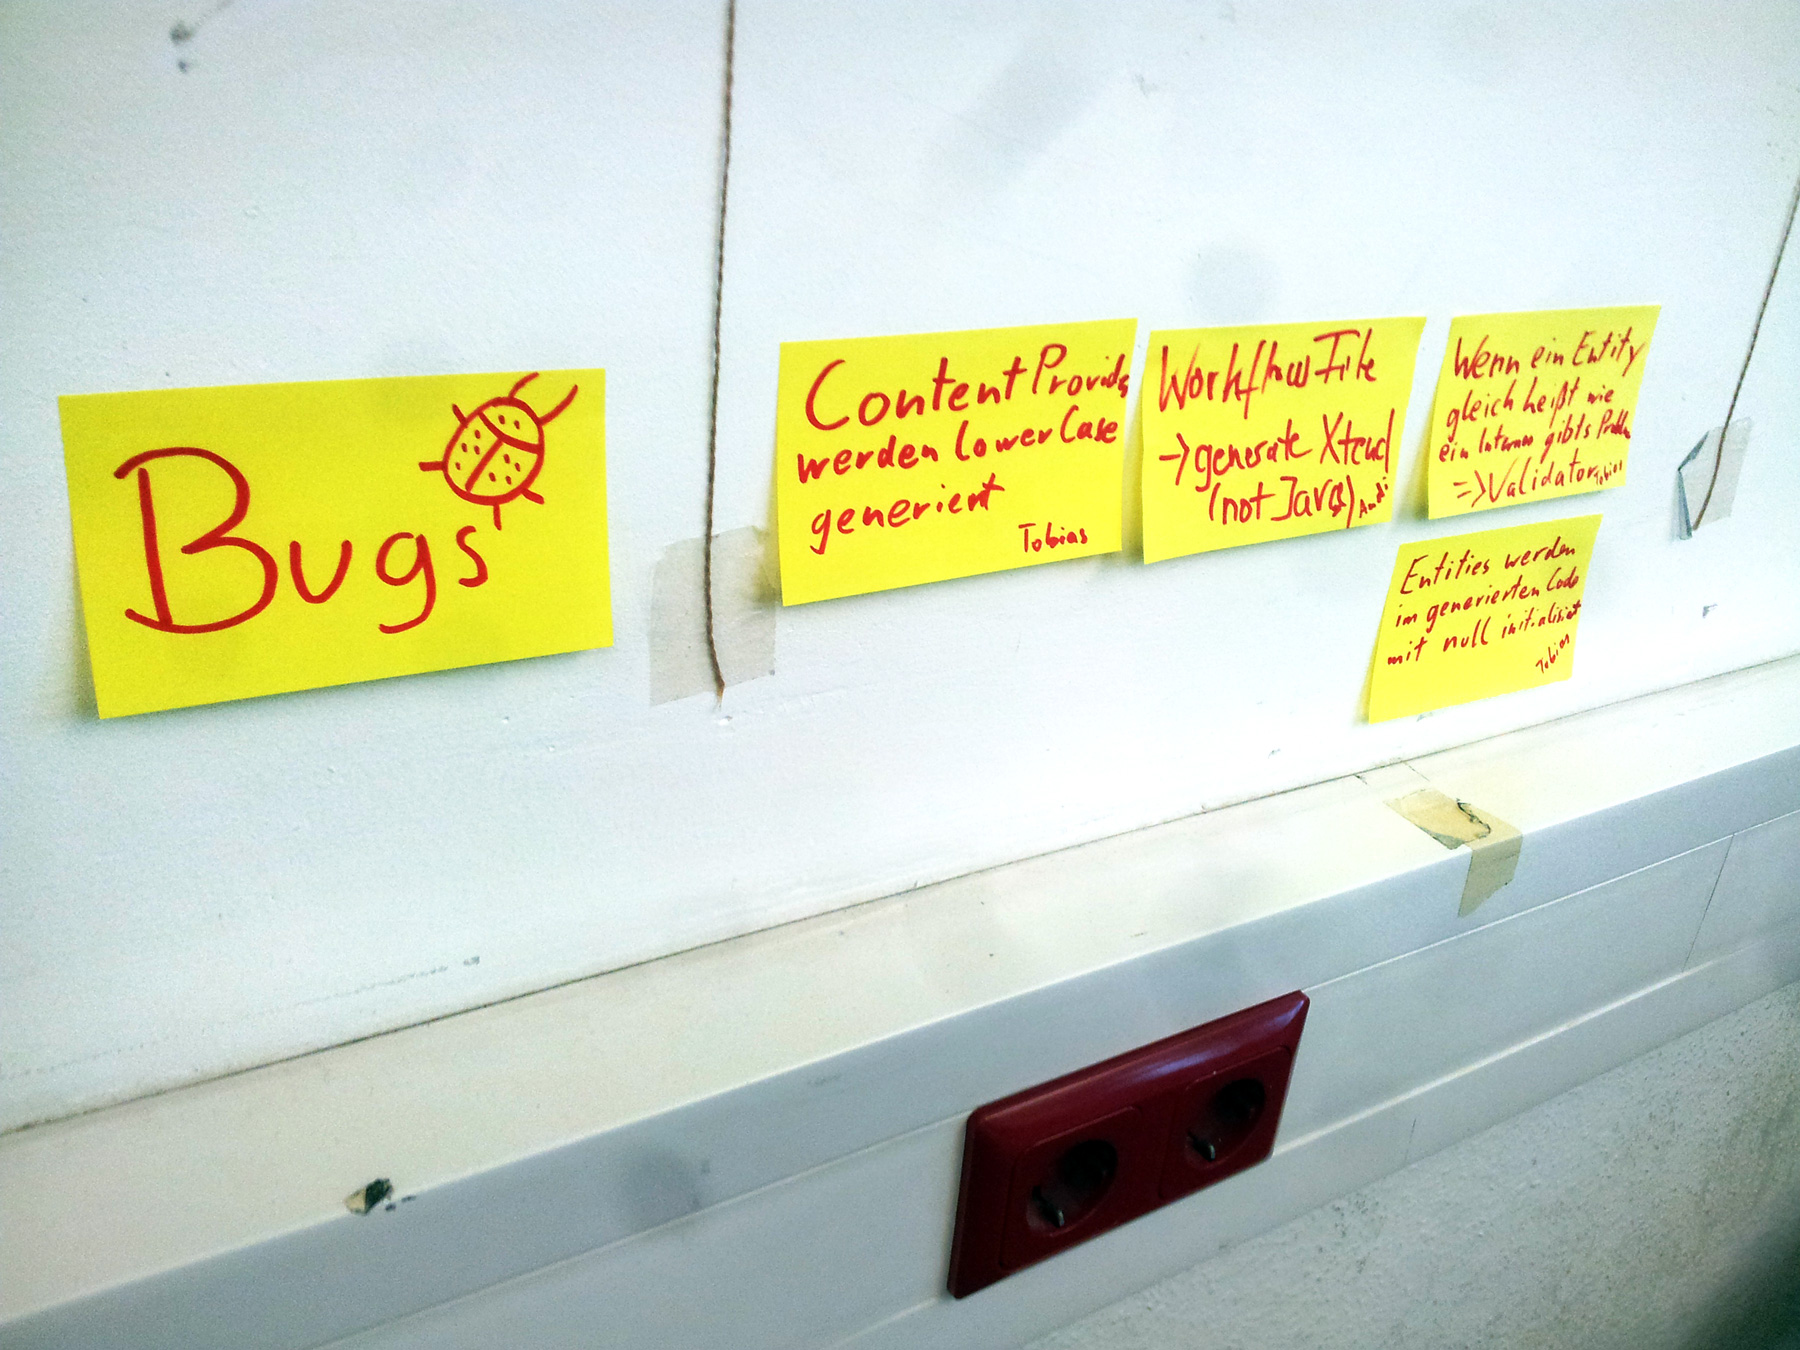
\includegraphics[width=.85\textwidth]{images/bugs}};
		\end{tikzpicture}
    \end{center}
\end{frame}

%-----------------------------------------------------------------------------------

\begin{frame}[fragile]
    \frametitle{Bug Fixes}

\begin{itemize}
  \item Disable a button \tiny{(e.g., "Previous" button in first view)}  
\end{itemize}

\begin{center}
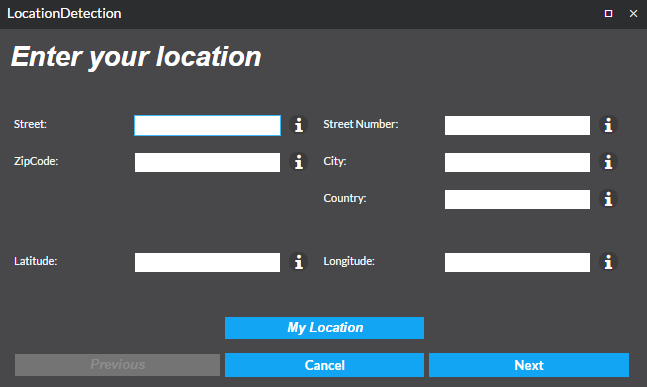
\includegraphics[width=0.6\textwidth] {images/disabled-previous-button.png}
\end{center}

\vspace{-1ex}

\begin{lstlisting}[basicstyle=\footnotesize\ttfamily]
Button MyPreviousBtn { 
  style button text "Previous" disabled true
}
\end{lstlisting}

\end{frame}	

%-----------------------------------------------------------------------------------

\begin{frame}
\frametitle{Story Cards}
\begin{center}
	\begin{tikzpicture}[
		line/.style= {pantone396!50!black},
		lbl/.style= {}
	]
		\draw[fill=pantone396!10!white, draw=pantone396] (0,0) rectangle (9, 6);
		\draw[line] (0, 2) -- (9, 2);
		\foreach \x in {1.5, 4.5, 7.5}
			\draw[line, dashed] (\x, 0) -- (\x, 2);
		\foreach \x in {3, 6}
			\draw[line, ] (\x, 0) -- (\x, 2);
		
		\node[lbl] at (1.5, 2.25) {\scriptsize{Implementation\vphantom{Aq}}};
		\node[lbl] at (4.5, 2.25) {\scriptsize{Tests\vphantom{Aq}}};
		\node[lbl] at (7.5, 2.25) {\scriptsize{Documentation\vphantom{Aq}}};
		
		\node[] at (4.5, 4) {\Large{Task Description}};
		
		\node at (0.75, 1.1) {\LARGE{\textbf{\checkmark}}};
		\node at (3.75, 1.1) {\LARGE{\textbf{\checkmark}}};
		
		\foreach \x in {0.75, 3.75, 6.75}
			\node at (\x, 0.2) {\tiny{DONE}};
		\foreach \x in {2.25, 5.25, 8.25}
			\node at (\x, 0.2) {\tiny{REVIEWED}};
			
		\node[overlay, inner sep = 0, draw, rotate=6] at (7.5, 5.75) {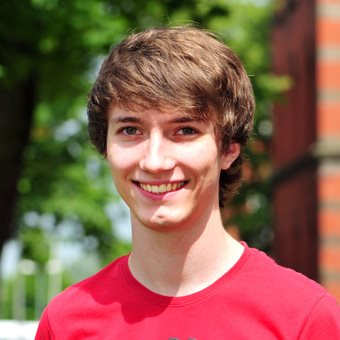
\includegraphics[width=1.75cm]{images/malte}};
		
	\end{tikzpicture}
\end{center}
\end{frame}

%-----------------------------------------------------------------------------------

\begin{frame}
    \frametitle{Continuous Integration with Jenkins}
    
    \begin{figure}
    	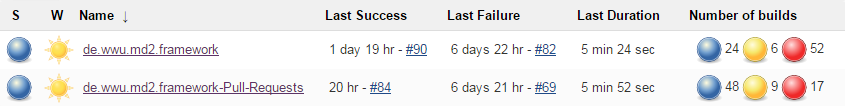
\includegraphics[width= 0.9\linewidth]{images/jenkins-jobs.png}
    \end{figure}
    
    \vspace{-1ex}
    
    \begin{itemize}
       \item \texttt{de.wwu.md2.framework}
       \begin{itemize}
           \item builds every time the \texttt{mapapps} branch is updated
       \end{itemize}
       \item \texttt{de.wwu.md2.framework-Pull-Requests} 
       \begin{itemize}
           \item builds for each pull request
           \item merged with current \texttt{mapapps} branch
       \end{itemize}
    \end{itemize}
\end{frame}

%-----------------------------------------------------------------------------------

\begin{frame}[plain]
\frametitle{Test Trend Chart: \texttt{mapapps} branch}
\plainnumber
\begin{center}
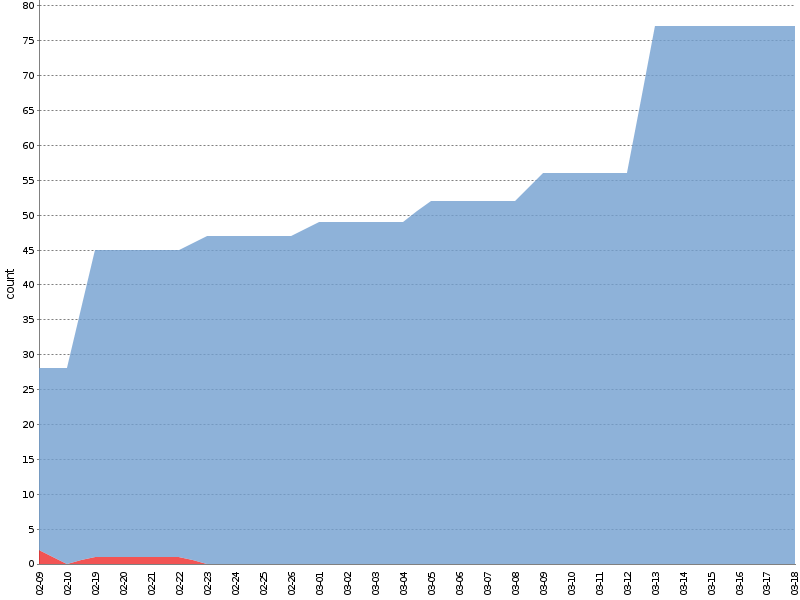
\includegraphics[width=1\textwidth] {images/test-trend-chart-md2-framework.png}
\end{center}
\end{frame}

%-----------------------------------------------------------------------------------

%\begin{frame}[plain]
%\frametitle{Test Trend Chart: pull requests}
%\plainnumber
%\begin{center}
%\includegraphics[width=1\textwidth, clip = true] %{images/test-trend-chart-md2-pull-requests.png}
%\end{center}
%\end{frame}

%-----------------------------------------------------------------------------------



